% ===========================================================================================================
% Backup

\section*{Backup Slides}

\begin{frame}{Security concepts}
    \begin{table}
        \centering
        \caption[Distinction between security concepts]{
            Distinction between security concepts based on areas of operations (derived from \cite{NawrockiWSKS2016}).
        }
        \begin{tabular}{l|lll}
            \toprule
            \textbf{Objective}        & \textbf{Prevention} & \textbf{Detection} & \textbf{Reaction} \\ \hline
            Honeypot                  & +                   & ++                 & +++               \\
            Firewall                  & +++                 & ++                 & +                 \\
            Intrusion Detection Sys.  & +                   & +++                & +                 \\
            Intrusion Prevention Sys. & ++                  & +++                & ++                \\
            Anti-Virus                & ++                  & ++                 & ++                \\
            Log-Monitoring            & +                   & ++                 & +                 \\
            Cybersecurity Standard    & +++                 & +                  & +                 \\
            \bottomrule
        \end{tabular}
        \label{tab:honeypots-security-concepts}
    \end{table}
\end{frame}

\begin{frame}{Value of Honeypots}
    \begin{columns}[T]
        % Column 1
        \begin{column}{0.49\textwidth}
            \begin{center}
                \textbf{Advantage}
            \end{center}
            \begin{itemize}
                \item \textit{Data Value}
                \item \textit{Resources}
                \item \textit{Simplicity}
                \item \textit{Return on Investment}
                %\item \textit{Independent of Workload}
                %\item \textit{Zero-Day-Exploit Detection}
                %\item \textit{Flexibility}
                %\item \textit{Reduced False Positives and Negatives}
            \end{itemize}
        \end{column}
        \begin{column}{.02\textwidth}
            \rule{.1mm}{0.7\textheight}
        \end{column}
        % Column 2    
        \begin{column}{0.49\textwidth}
            \begin{center}
                \textbf{Disadvantage}
            \end{center}
            \begin{itemize}
                \item \textit{Narrow Field of View}
                \item \textit{Fingerprinting}
                \item \textit{Risk to the Environment}
            \end{itemize}
        \end{column}
    \end{columns}
\end{frame}

\begin{frame}{Honeynets}
    Advantage:
    \begin{itemize}
        \item dedicated network full of honeypots
        \item allows easier usage of real machines
        \item learn about attacker's network communication
    \end{itemize}
    Downside: complex to deploy and maintain
\end{frame}

\begin{frame}{Example of Honeynets}
    \begin{figure}
        \centering
        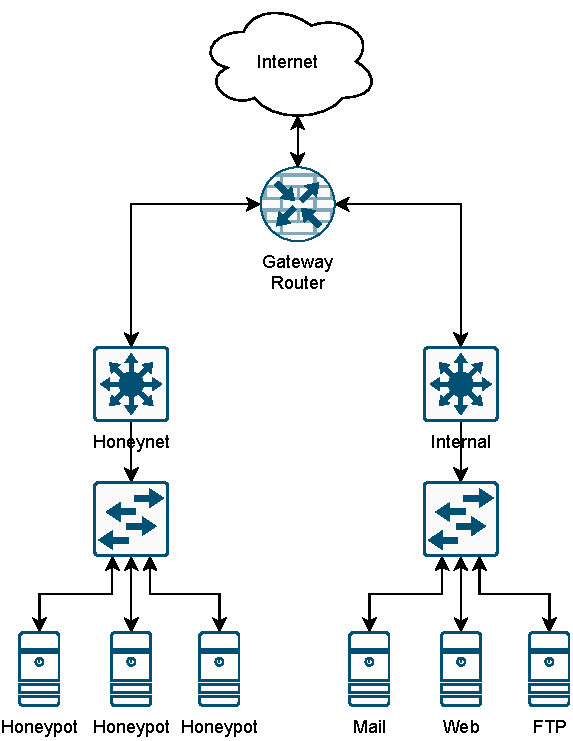
\includegraphics[width=0.5\columnwidth]{img/honeynet-example.pdf}
        \caption[Example of honeynets in a network]{
            Example of honeynets in a network (derived from \cite{Spitzner2003}).
        }
    \end{figure}
\end{frame}

\begin{frame}{Legal Issues}
    \begin{block}{General}
        A honeypot has a legal ground of legitimate interest to store and process personal data.\\
        The principle of data minimization has to be applied.\\
        Any published data needs to be anonymized.\\
        \cite{sokol2017}
    \end{block}
    Honeypots collect:
    \begin{itemize}
        \item content data
        \item transactional data 
    \end{itemize}
\end{frame}

\begin{frame}{T-Pot}
    \begin{figure}
        \centering
        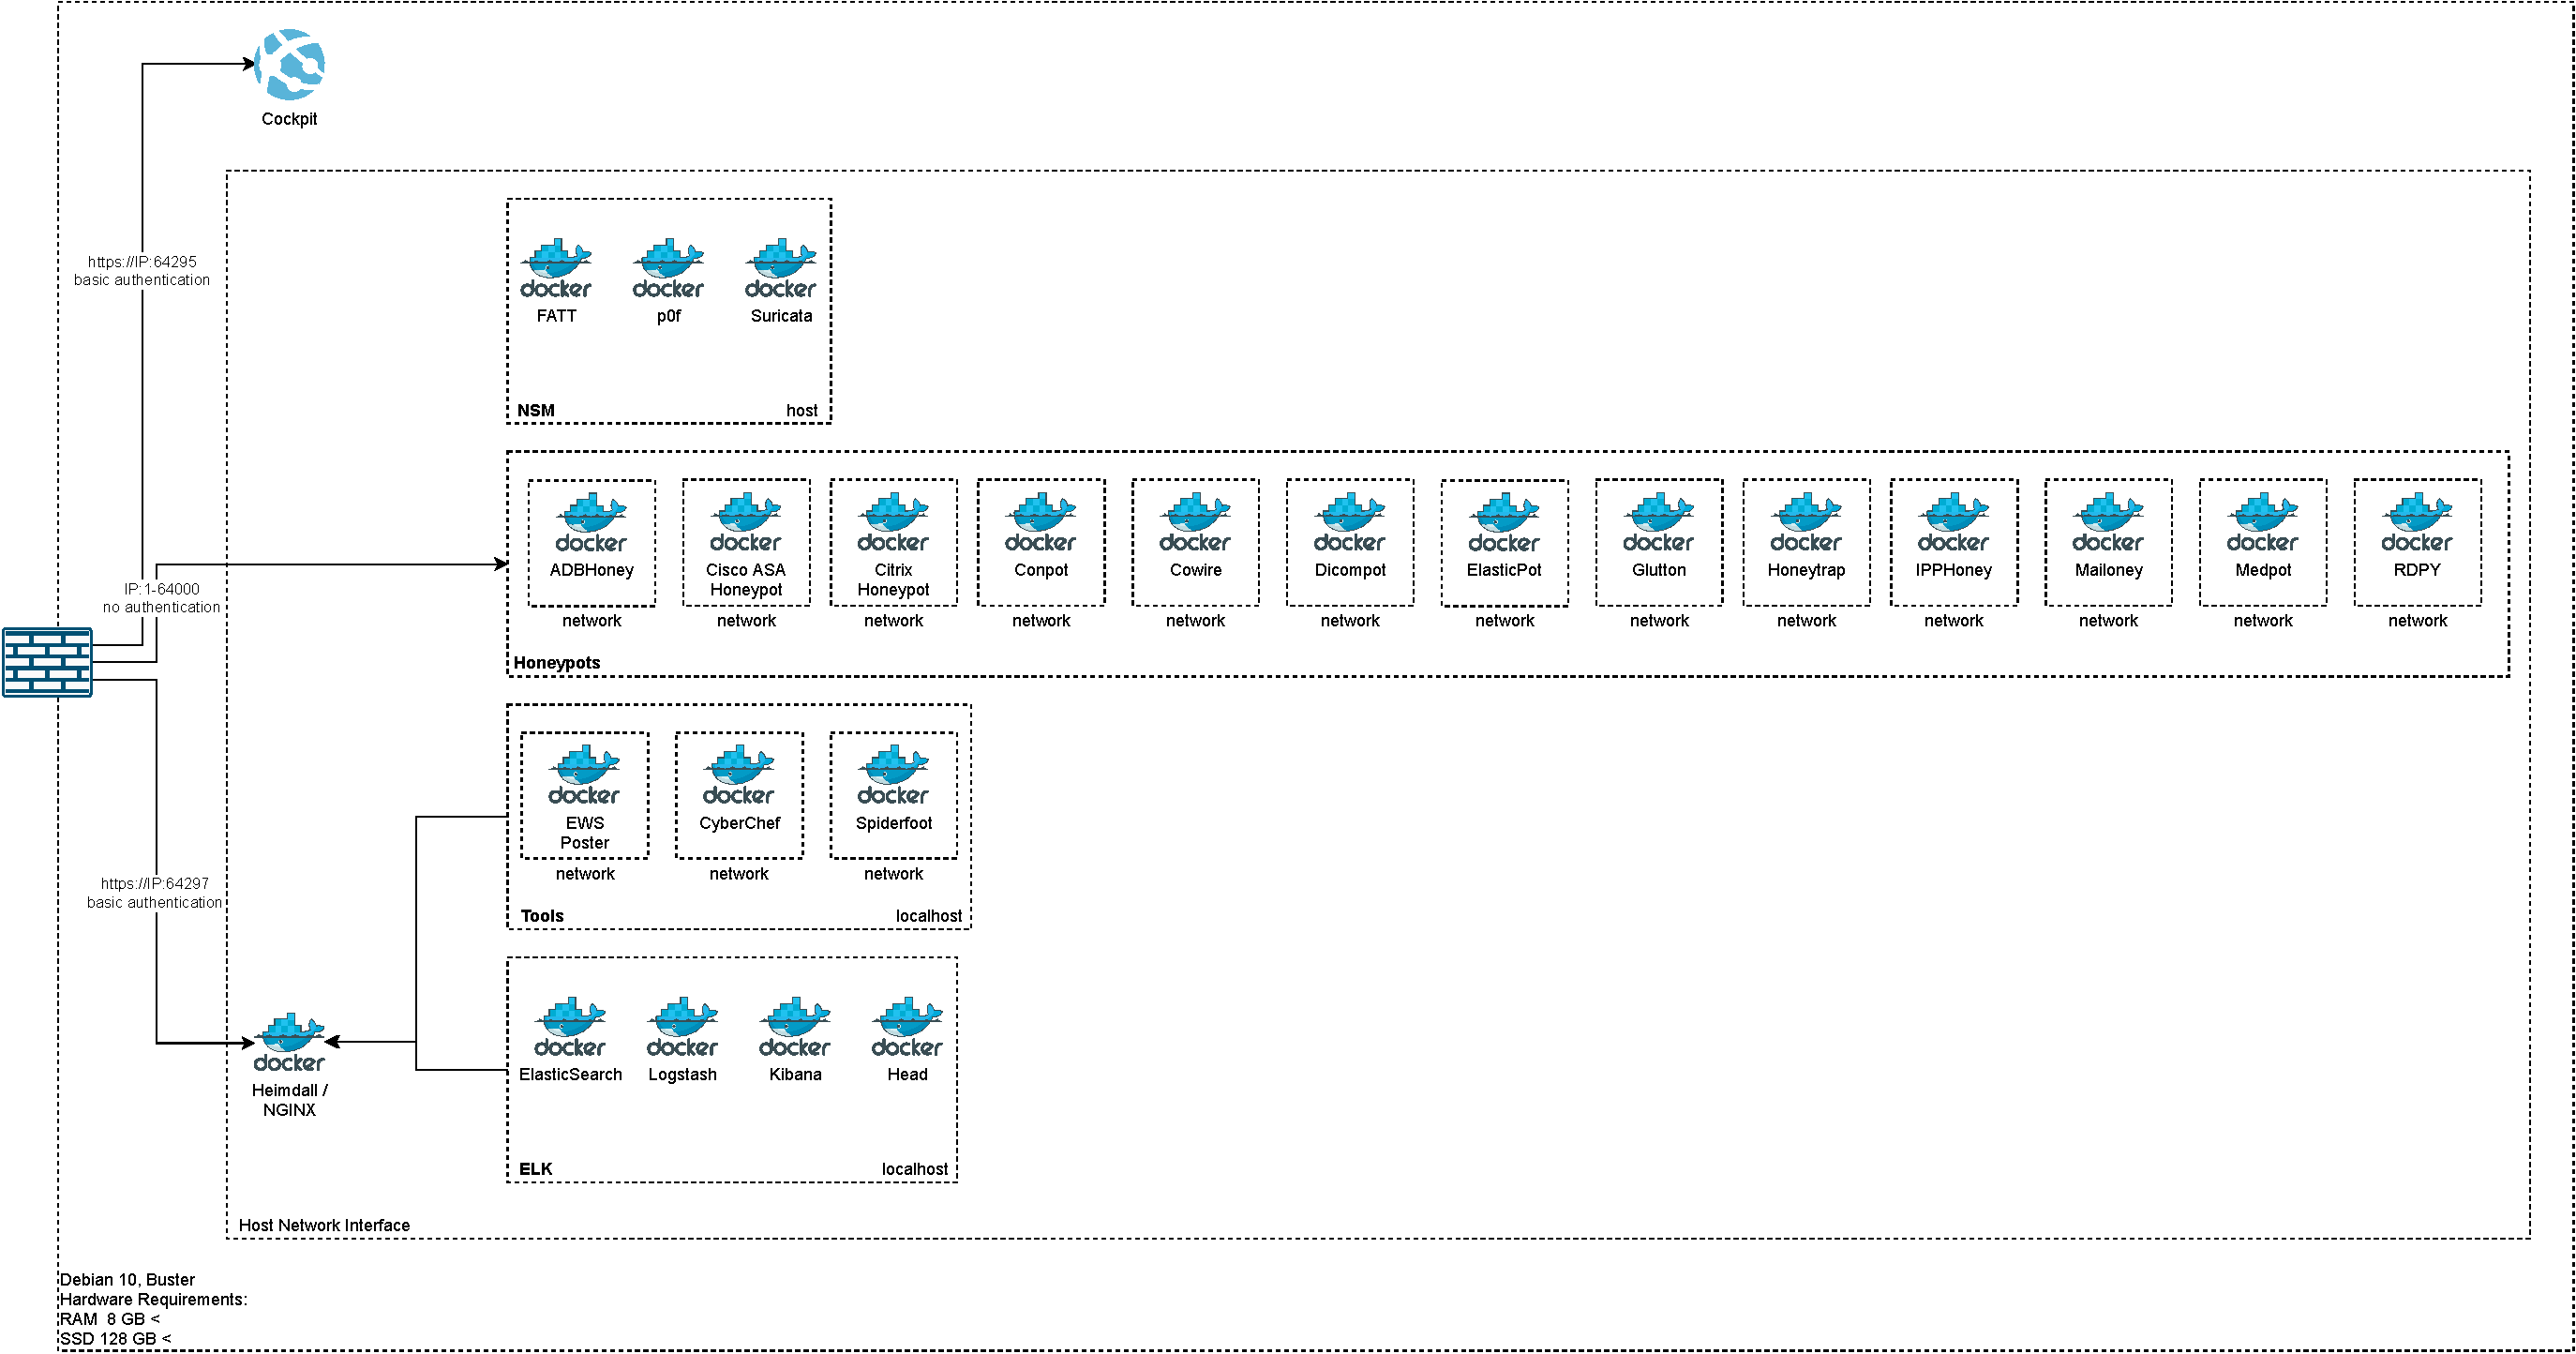
\includegraphics[width=\columnwidth]{img/tpot-architecture.pdf}
    \end{figure}
\end{frame}

\begin{frame}{Infrastructure-as-a-Service (IaaS)}
    \begin{columns}[T]
        \begin{column}{0.5\textwidth}
            \begin{center}
                Overall
            \end{center}
            \begin{itemize}
                \item Low-level abstraction to consumers
                \item Usage of IT infrastructure capabilities
                \item Depend on virtualization due to the integration or decomposition of physical resources
            \end{itemize}
        \end{column}
        % Column 2
        \begin{column}{.02\textwidth}
            \rule{.1mm}{0.7\textheight}
        \end{column}
        % Column 1
        \begin{column}{0.5\textwidth}
            \begin{center}
                Differences
            \end{center}
            \begin{itemize}
                \item Various pricing models
                \item Offer apps and tools for maintenance
                \item Not necessarily abide EU law
            \end{itemize}
        \end{column}
    \end{columns}
\end{frame}

\begin{frame}{Kelly et. al's findings}
    Recent study for AWS, GCP, and Azure\\
    in East US, West Europe, and Southeast Asia
    \begin{itemize}
        \item \numprint{55000} attacks per day
        \item In total $1.17$ mio. attacks
        \item Most attacked honeypots: Glutton, Cowrie, Dionaea
    \end{itemize}
\end{frame}

\begin{frame}{Kelly et. al's findings}
    Most important
    \begin{itemize}
        \item Focus on remote desktop software
        \item Attacks origin from Vietnam, Russia, the United States, and China
        \item Information gathering about PU architecture, scheduled tasks, and privilege escalation
    \end{itemize}
\end{frame}

\begin{frame}{Internal Network}

\end{frame}

\begin{frame}{MADCAT}
    \begin{figure}
        \centering
        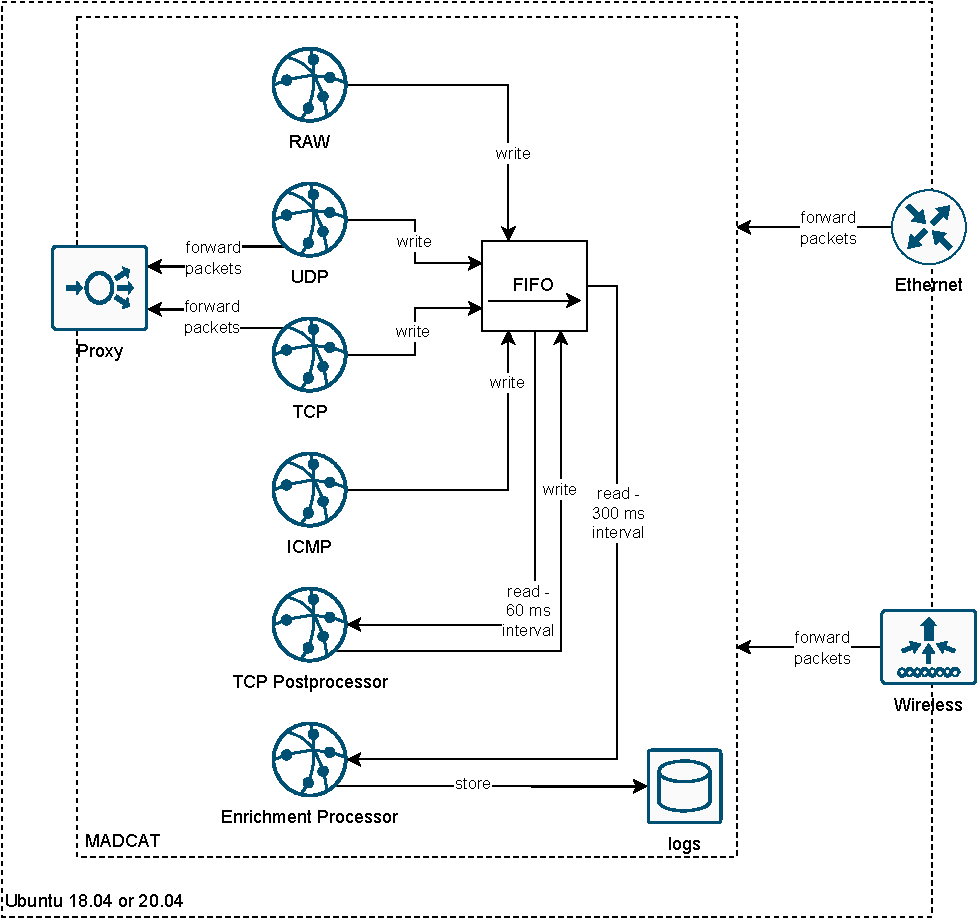
\includegraphics[width=0.7\columnwidth]{img/heicat_architecture.pdf}
        \caption[MADCAT architecture]{
            MADCAT architecture
        }
    \end{figure}
\end{frame}

\begin{frame}{TCP/IP}

\end{frame}

\begin{frame}{OpenSSH}
    \begin{figure}
        \centering
        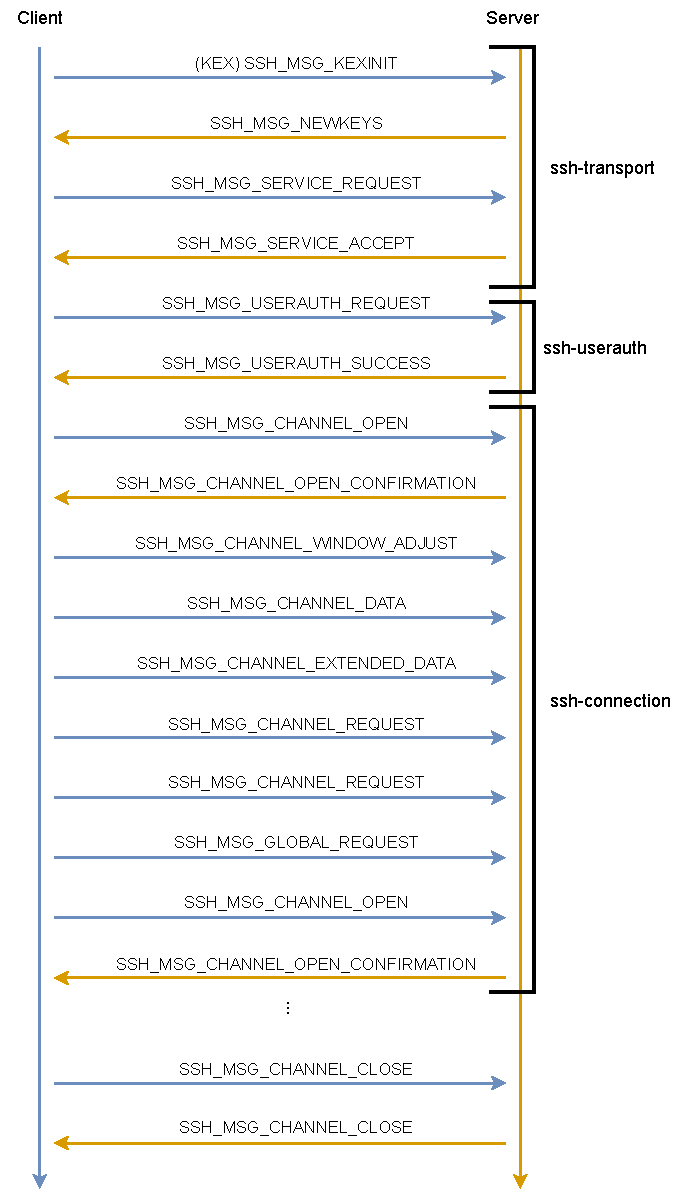
\includegraphics[width=0.35\columnwidth]{img/ssh-flow-diagram.pdf}
        \caption[OpenSSH sample session flow diagram]{
            OpenSSH sample session flow diagram (derived from \cite{openssh2007}).
        }
    \end{figure}
\end{frame}